\documentclass[12pt,fleqn]{article}\usepackage{common}
\begin{document}

Felzenszwalb Clustering

Load up data

\begin{minted}[fontsize=\footnotesize]{python}
import pandas as pd
syn = pd.read_csv("synthetic.txt",names=['a','b'],sep="   ")
print syn.shape
data = np.array(syn)
\end{minted}

\begin{verbatim}
(3000, 2)
\end{verbatim}

It looks like this

\begin{minted}[fontsize=\footnotesize]{python}
plt.scatter(data[:,0],data[:,1])
plt.savefig('test_02.png')
\end{minted}

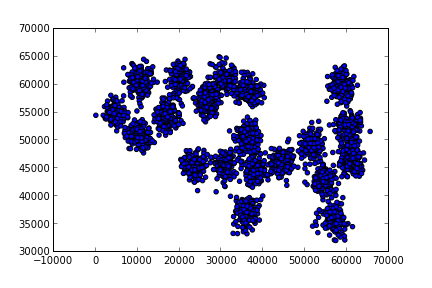
\includegraphics[height=6cm]{test_02.png}

\begin{verbatim}
(3000, 2)
\end{verbatim}

Create pairwise Euclidian distances

\begin{minted}[fontsize=\footnotesize]{python}
from sklearn.metrics.pairwise import euclidean_distances
X = euclidean_distances(data, data)
print X.shape
print X[1,2]
\end{minted}

\begin{verbatim}
(3000, 3000)
622.540761718
\end{verbatim}

Remove distances that are too big, so we can create a sparse array

\begin{minted}[fontsize=\footnotesize]{python}
import scipy.sparse as sps
from scipy.io import mmwrite, mmread
print X.shape
X2 = X.copy()
print X2.mean(), X2.std()
X2[X > 2000] = 0.0
print X2.shape
X3 = sps.lil_matrix(X2)
print X3.shape
print 'before triu', len(X3.nonzero()[0])
X4 = sps.triu(X3)
print  'after triu', len(X4.nonzero()[0])
\end{minted}

\begin{verbatim}
(3000, 3000)
23275.2891376 13430.4720182
(3000, 3000)
(3000, 3000)
before triu 174020
after triu 87010
\end{verbatim}

Take only upper triangular part of the matrix because it is symmetric, cuts
the number of non-zero cells by half,

\begin{minted}[fontsize=\footnotesize]{python}
import scipy.sparse as sps
from scipy.io import mmwrite, mmread
mmwrite('/tmp/syndist', X4)
\end{minted}

\begin{minted}[fontsize=\footnotesize]{python}
!../felzclust/felzclust /tmp/syndist.mtx 25000 20  > /tmp/out
df = pd.read_csv('/tmp/out',sep=';')
syn['cluster'] = df['cluster']
print len(syn['cluster'].unique()), 'clusters found'
print syn[:5]
\end{minted}

\begin{verbatim}
14 clusters found
       a      b  cluster
0  54620  43523      238
1  52694  42750      238
2  53253  43024      238
3  54925  42624      238
4  54973  43980      238
\end{verbatim}

\begin{minted}[fontsize=\footnotesize]{python}
import random
for clust in syn['cluster'].unique():
    tmp = np.array(syn[syn['cluster'] == clust][['a','b']])
    plt.scatter(tmp[:,0], tmp[:,1], c=np.random.rand(3,1))
plt.savefig('test_01.png')
\end{minted}


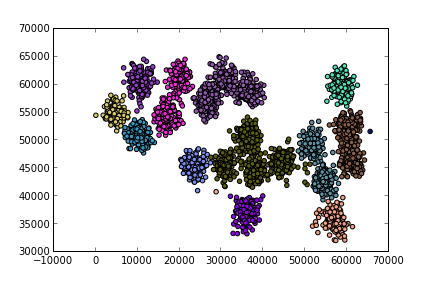
\includegraphics[height=8cm]{test_01.png}









\end{document}
